\documentclass[12pt, a4paper]{report}
\usepackage{graphicx}
\usepackage{subcaption}
\usepackage{tabto}
\usepackage{hyperref}

%\title{Compiler Construction Report}
%\author{Nguyen Ngoc Lam \\ICT.02-K61 \\
%		Instructor: Nguyen thi Thu Huong}
%\date{\today}



\begin{document}
	%\maketitle
	\begin{titlepage}
		\begin{center}
       		\vspace*{1cm}
 			
 			\Huge
       		\textbf{Compiler Construction Report}
 
       		\vspace{0.5cm}Instructor: Nguyen thi Thu Huong
 
       		\vspace{1.5cm}
 
       		\textbf{Nguyen Ngoc Lam \\ICT.02-K61 }
 
       		\vfill
 
 			
 			
\includegraphics[width=0.4\textwidth]{university.png}      		
 			\normalsize
       		\vspace{0.8cm}
 
      		
 
       		University Name: Hanoi University of Science and Technology\\
       		Date: \today
 
   		\end{center}
	\end{titlepage}
	\tableofcontents
	\newpage
	\chapter{AN OVERVIEW OF COMPILER}
	\newpage
		\section{Task of a compiler}
			\tab In simple words, A compiler is a computer program (or set of programs) that transforms source code written in a programming language (the source language) into another computer language (the target language, often having a binary form known as object code). The most common reason for converting a source code is to create an executable program. Another critical goal of a compiler is to report errors in source code to developers.\\
			\tab See more at: \url{http://en.wikipedia.org/wiki/Compiler}
			\begin{figure}[h]
				\centering
				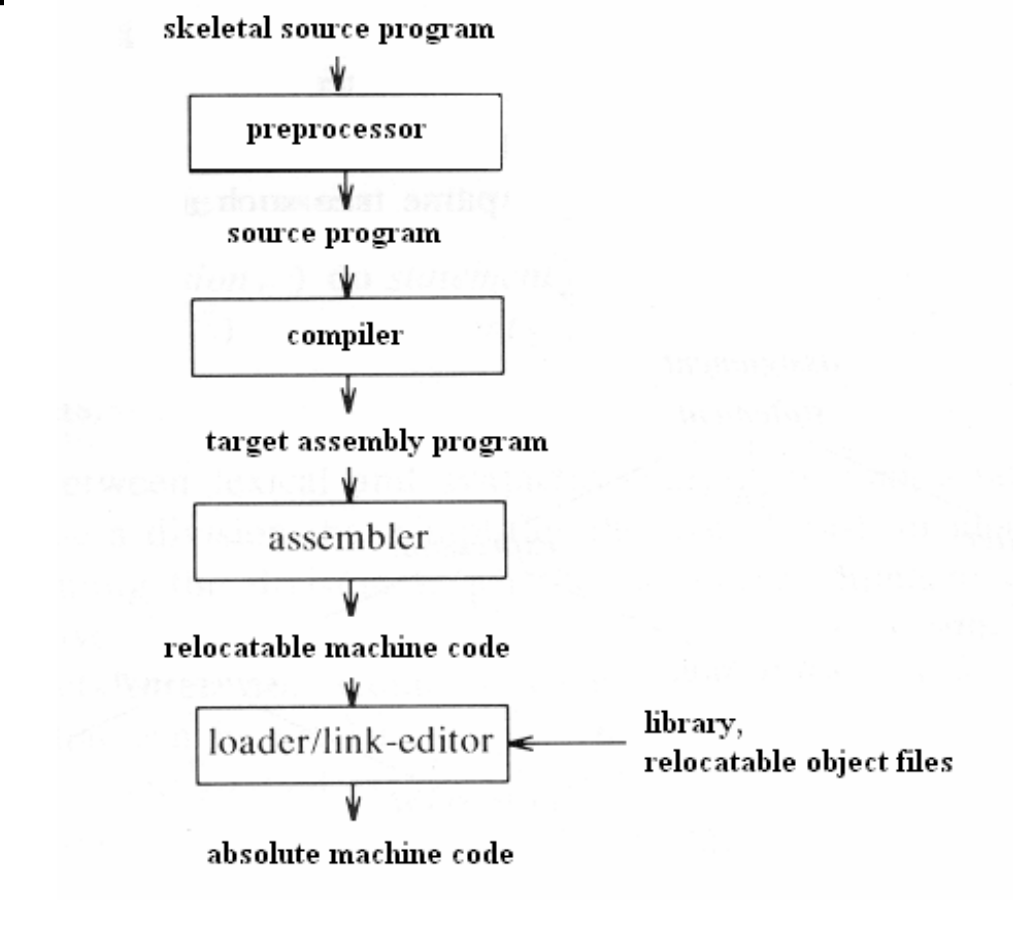
\includegraphics[width=0.95\textwidth]{compilerinLangproc.png}
				\caption{Context of a compiler in a language processor}
				\label{fig:inContext}
			\end{figure}
		\section{COMPONENTS OF A COMPILER}		
			\tab A compiler can be divided into 4 main parts:
			\begin{itemize}
				\item Lexical analyzer
				\item Syntax analyzer
				\item Semantic analyzer
				\item Code generator
			\end{itemize}
			\begin{figure}[h]
				\centering
				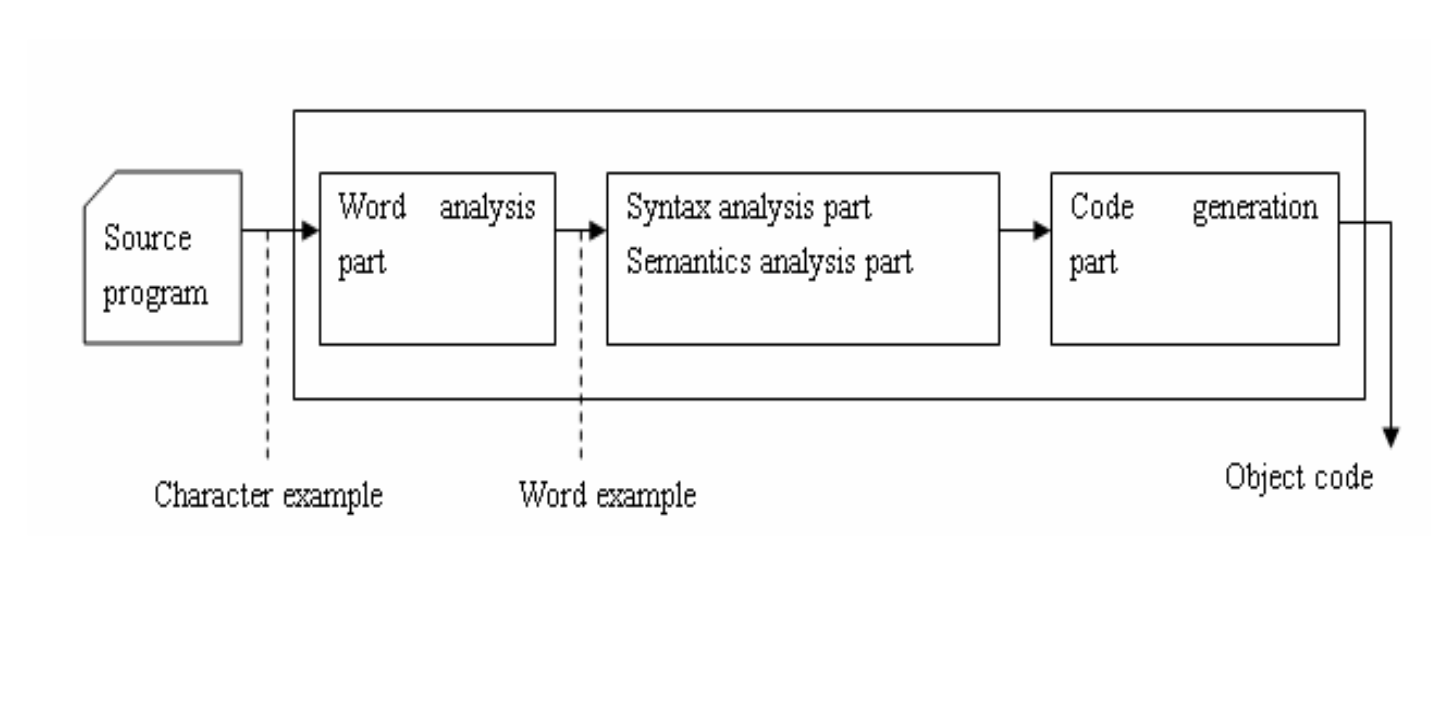
\includegraphics[width=0.95\textwidth]{compileStage.png}
				\caption{Parts of a compiler}
				\label{fig:stage}
			\end{figure}
		\section{Steps of the compiling process}
			\tab A compiler is divided into several interrelated processes,  in each process, source program is translated from a specific form to another form of representation. For better understanding, see figure \ref{fig:decomp}
			\begin{figure}[h!]
				\centering
				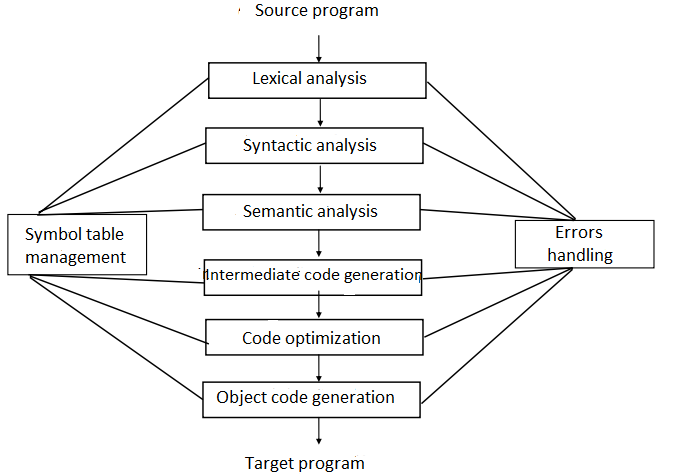
\includegraphics[width=0.95\textwidth]{step.png}
				\caption{A typical decomposition}
				\label{fig:decomp}
			\end{figure}
			\newline
			\tab Consider an example in KPL:
			\begin{equation}
				\label{eq:1}
				Sum := initial + increment * 50
			\end{equation}
			\subsection{Lexical analyzer}
				\tab Lexical analysis \footnote{Note that in the process of lexical analysis, the space, tabulator, and the comments (in KPL // or /**/) will be neglected.} is the process of converting a sequence of characters into a sequence of tokens, i.e. meaningful character strings. A program or function that performs lexical analysis is called a lexical analyzer, lexer, tokenizer, or scanner, though "scanner" is also used for the first stage of a lexer. \\
				\tab A token is a string of one or more characters that is significant as a group. The process of forming tokens from an input stream of characters is called tokenization. The characters that form a token are called a lexeme. 
				See more at \url{http://en.wikipedia.org/wiki/Lexical_analysis}
				\newline
				The process of lexical analysis will occur as follows: the scanner will read character-by-character input stream to generate tokens. So the result of the example \ref{eq:1} will be:
				\begin{enumerate}
					\item Identifier (sum)
					\item Symbol that represents assignment  (:=)
					\item Identifier (initial)
					\item Symbol that represents addition (+)
					\item Identifier (increment)
					\item Symbol that represents multiplication (*)
					\item Number (50)
				\end{enumerate}
			\subsection{Syntax analysis}
				\tab Syntactic analysis (also called parsing) is the process of analysing a string of tokens, conforming to the rules of a formal grammar or not. The program that performs parsing is called the syntactic analyser or simply parser. The output of parsing is the parse tree, or error. Parsing is based on grammar provided to build parse tree.
The most important part of building a compiler is the task of building a grammar that generates structure of a program and cannot be ambiguous. An ambiguous grammar will produce more than one parse tree, therefore must be forbidden. \\
The example \ref{eq:1} will produce following parse tree:
				\begin{figure}[h]
					\centering
					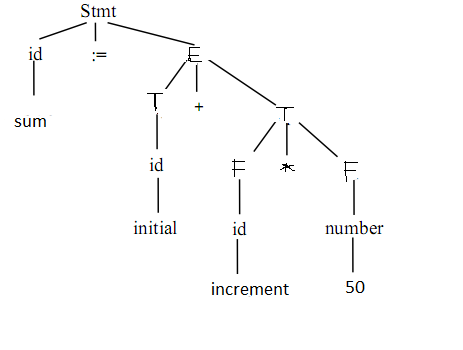
\includegraphics[width=0.95\textwidth]{pt.png}
					\caption{Parse tree of \ref{eq:1}}
					\label{fig:parseTree}
				\end{figure}
			\newpage
			\subsection{Semantic analysis}
				\tab Semantic analysis is the phase in which the compiler adds semantic information to the parse tree and builds the symbol table. This phase performs semantic checks such as type checking (checking for type errors), or object binding (associating variable and function references with their definitions), or definite assignment (requiring all local variables to be initialized before use), rejecting incorrect programs or issuing warnings. Semantic analysis usually requires a complete parse tree, meaning that this phase logically follows the parsing phase, and logically precedes the code generation phase.\\ \\
				\tab An important part of semantic analysis is type checking and variable scope checking. In this step, compiler will check, according to specification from source language. In additional, semantic analyser will use symbol table to store information about every identifier, which will generate information about the position of storing identifiers,type  and scope of them in program or procedure that include them, or if an identifier is name of function or procedure, it will store information about number and type of parameters, return type, etc.
			\subsection{Intermediate code generation}
				\tab After the phase of semantic analysis, some compiler will generate an intermediate representation of source program, known as intermedia code. We can consider this representation as a program for an abstract virtual machine. They have three important properties: easy to generate, easy to translate into object code and machine-independent. Usually, compiler use three-address codes. Three-address codes are codes that accept at most three parameters, one operator (except assignment). So before generation of these codes, compiler need rules of operator precedence, e.g * before +. Example \ref{eq:1} gives the following intermediate code:
				\begin{itemize}
					\item[] $$T1: = 50;$$
					\item[] $$T2:= ID3 * T1;$$
					\item[] $$T3 := ID2 + T2;$$
					\item[] $$ID1:= T3;$$
				\end{itemize}
			\subsection{Code optimization}
				\tab In this phase, code optimizator will try to optimize the intermediate code into equivalent one with faster execution. 
For example, the example \ref{eq:1} can be optimized as:
				\begin{itemize}
					\item[] $$T1: = ID3 * 50;$$
					\item[] $$ID1:= ID2 + T1;$$
				\end{itemize}
				\tab There is a significant difference between the amount of optimization codes done by different compiler. In some compiler called “optimize-focused compiler”, a conspicuous proportion of time devoted to this phase. However, there are also some optimization method that can decrese lots of execution time of source program without wasting too much time compiling.
			\subsection{Object code generation}
				\tab This is the final phase of compiler. Input of a object code generator is the intermediate code and output is the target program. There are a number of factors that affect the design of an object code generator such as: memory management, resource allocation and the sequence of code execution.
		\section{SUMMARY}
			\tab In order for a computer to understand and execute a program written in a high-level programming language, we need a compiler to translate source program to target program in object codes. This chapter has presented an overview of a compiler in general, including lexical analysis, syntax analysis,  semantic analysis, intermediate code generation, code optimization and object code generation. Output of the preceding phases are always input of the following phases, i.e, output of a scanner (tokens) will be input of the parser, output of the parser (parse tree) will be input of the semantic analyzer, etc.
	
	\chapter{LEXICAL ANALYSER FOR KPL}
	\newpage
	\large\textbf{In a compiler, the program that perform lexical analysis is called the scanner.}
	
		\section{TASK OF A SCANNER}
			\begin{itemize}
				\item Neglect meaningless character: space, tabulalor, EOF, CR, LF, comments.
				\item Detect invalid symbols: @, ! (stand-alone), etc
				\item Detect and produce tokens: identifiers, keywords, numbers, literals, special characters, etc.
			\end{itemize}
		\section{TOKENS IN KPL}
			\begin{itemize}
				\item Identifier: variable name, constant names, type names, function names, procedure names:
				\begin{itemize}
					\item Start with letter or underscore: a-z, A-Z, '\_'
    				\item Others are letter, underscore or numbers
				\end{itemize}
				\item Keywords: PROGRAM, CONST, TYPE, VAR, PROCEDURE, FUNCTION, BEGIN, END, ARRAY, OF, INTEGER, CHAR, CALL, IF, ELSE, WHILE, DO, FOR, TO
				\item Operators: := (assign), + (addition), - (subtraction), * (multiplication), / (division), = (comparison of equality), != (comparison of difference), $>$ (comparison of greaterness), $<$ (comparison of lessness), $>=$ (comparison of greaterness or equality), $<=$ (comparison of lessness or equality)
				\item Special characters ; (semicolon), . (period), : (colon), , (comma), ( (left parenthesis), ) (right parenthesis), \' \, (singlequote), (. and .) to specify indexes in arrays and (*, *) to indicate comments
				\item Others: integer number, string literals,\ldots
			\end{itemize}
		\section{DATA STRUCTURE IN KPL}
			\begin{enumerate}
				\item \textbf{Data structure to store valid characters in KPL : $space,\, letters,\, numbers,\, +,\, -,\, *,\, /,\, <,\, >,\, ! ,\, =,\, , ,\, . ,\, : ,\, ; ,\, ‘ ,\, (. ,\, .)$ others are invalid characters (CHAR\_ UNKNOWN)}\\ \newline
					typedef enum \{\\
          CHAR\_ SPACE, CHAR\_ LETTER, CHAR\_ DIGIT, CHAR\_ PLUS,\\            
          CHAR\_ MINUS, CHAR\_ TIMES, CHAR\_ SLASH, CHAR\_ LT, \\
          CHAR\_ GT, CHAR\_ EXCLAIMATION, CHAR\_ EQ, CHAR\_ COMMA,\\
          CHAR\_ PERIOD, CHAR\_ COLON, CHAR\_ SEMICOLON, \\  
          CHAR\_ SINGLEQUOTE, CHAR\_ LPAR, CHAR\_ RPAR,  \\
          CHAR\_ UNKNOWN  \\
      \} CharCode;
				\item \textbf{Stores token types in KPL:}\\ \newline
				typedef enum \{\\
            TK\_ NONE, TK\_ IDENT, TK\_ NUMBER, TK\_ CHAR, TK\_ EOF,\\
            KW\_ PROGRAM, KW\_ CONST, KW\_ TYPE, KW\_ VAR,\\
            KW\_ INTEGER, KW\_ CHAR, KW\_ ARRAY, KW\_ OF, \\
            KW\_ FUNCTION, KW\_ PROCEDURE,\\
            KW\_ BEGIN, KW\_ END, KW\_ CALL,\\
            KW\_ IF, KW\_ THEN, KW\_ ELSE,\\
            KW\_ WHILE, KW\_ DO, KW\_ FOR, KW\_ TO,\\

            SB\_ SEMICOLON, SB\_ COLON, SB\_ PERIOD, SB\_ COMMA,\\
            SB\_ ASSIGN, SB\_ EQ, SB\_ NEQ, SB\_ LT, SB\_ LE, SB\_ GT, SB\_ GE, \\
  	 SB\_ PLUS, SB\_ MINUS, SB\_ TIMES, SB\_ SLASH,\\
  	 SB\_ LPAR, SB\_ RPAR, SB\_ LSEL, SB\_ RSEL\\
       \} TokenType;
       			\item \textbf{Store information about each tokens:}
       				\begin{itemize}
       					\item string : content of token 
     					\item lineNo , colNo : position of  token, 
     					\item tokenType : type of token 
      					\item value : value of token if  a number.
					\end{itemize}
					typedef struct \{\\
           \textbf{char} string[MAX\_ IDENT\_ LEN + 1];\\
           \textbf{int} lineNo, colNo; // line and column of tokens\\
           \textbf{TokenType} tokenType;\\
           \textbf{int} value;\\
       \} \textbf{Token};      				  
			\end{enumerate}
		\section{FUNCTIONS IN KPL}
			\subsection{Details about functions}
				\begin{itemize}
					\item \textbf{void} skipBlank() : skip spaces.
      				\item \textbf{void} skipComment() : skip comments.
      				\item \textbf{Token*} readIdentKeyword() : read identifiers or keywords, return a pointer of Token type.
      				\item \textbf{Token*} readNumber() : read a integer number, return a pointer of Token type.
      				\item \textbf{Token*} readConstChar() : read a constant character, return a pointer of Token type.
      				\item \textbf{TokenType} checkKeyword(\textbf{char *}string) : check if the string is a keyword, return TOKEN\_ NONE if keyword.
      				\item \textbf{Token*} makeToken(\textbf{TokenType} tokenType, \textbf{int} lineNo, \textbf{int} colNo) : create a pointer to a token with predefined type and position.
      				\item \textbf{Token*} getToken() : read and return a token (can be invalid token: TOKEN\_ NONE).
          			\item \textbf{Token*} getValidToken() : read and return a valid token.
				\end{itemize}
			\subsection{Details about execution of a scanner}
				\begin{enumerate}
					\item Scanner is a finite automation. Everytime it return a token, the state will be 0.  When detects invalid characters, the state will be -1
					\item During the reading of input stream,  getToken() will be looped until meet (EOF)
					\item If detect
					\begin{itemize}
						\item spaces (CHAR\_ SPACE)  -$>$ skipBlank(), state will be 0,  -$>$ getToken(), \ldots
      					\item other tokens, that token will be passed to parser for the next phase of compiling process.
					\end{itemize}
				\end{enumerate}
				\begin{figure}[t!]
					\centering
					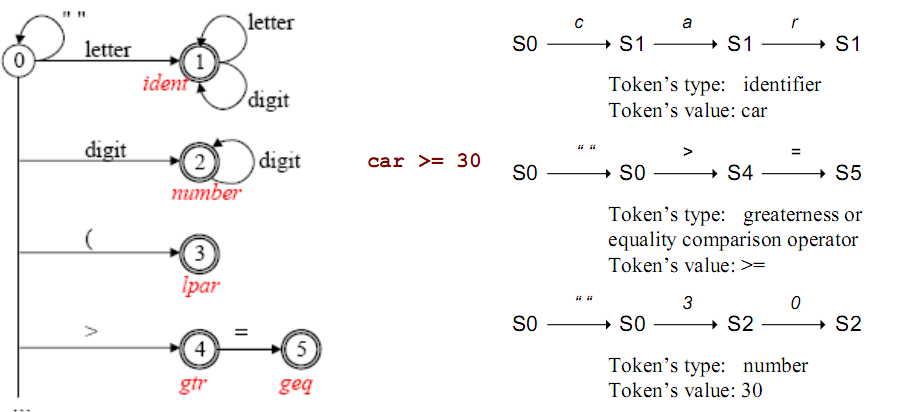
\includegraphics[width=0.95\textwidth]{execLex.png}
					\caption{Execution of a scanner}
					\label{fig:execLex}
				\end{figure}
	\chapter{SYNTACTIC ANALYSER FOR KPL}
	\newpage
		\section{Task of a syntatic analyser (parser)}
			\begin{itemize}
				\item Check the syntax of the program for errors
     			\item Produce parse tree for semantic analyser otherwise
			\end{itemize}
		\section{Syntax diagram and BNF grammar}
			\subsection{Syntax diagram}
				\begin{figure}[h]
					\centering
					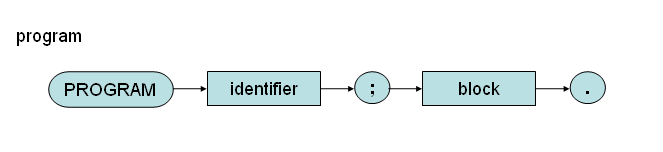
\includegraphics[width=\linewidth]{syn1.png}
					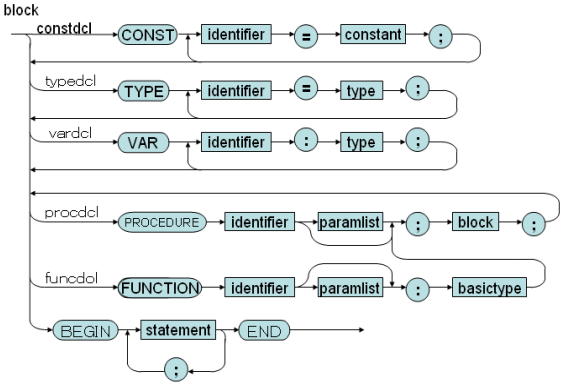
\includegraphics[width=\linewidth]{syn2.png}
					
					\caption{Syntax diagram 1.}
					\label{fig:syn1}
				\end{figure}
				\begin{figure}[hp]
					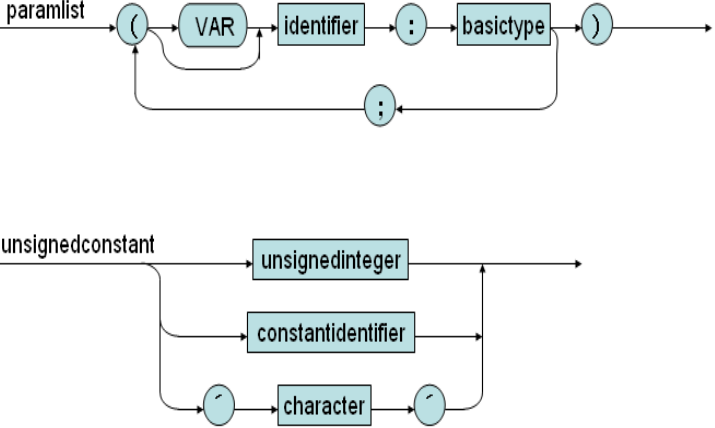
\includegraphics[width=\linewidth]{syn3.png}
					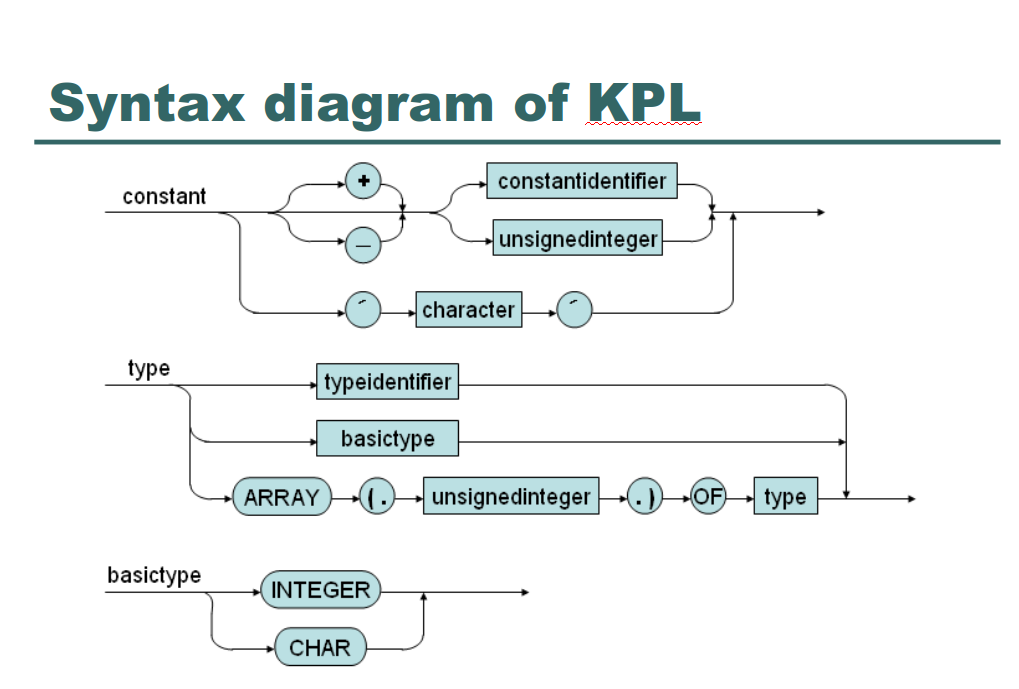
\includegraphics[width=\linewidth]{syn4.png}
					
					\caption{Syntax diagram 2.}
					\label{fig:syn2}
				\end{figure}
				\begin{figure}[hp]
					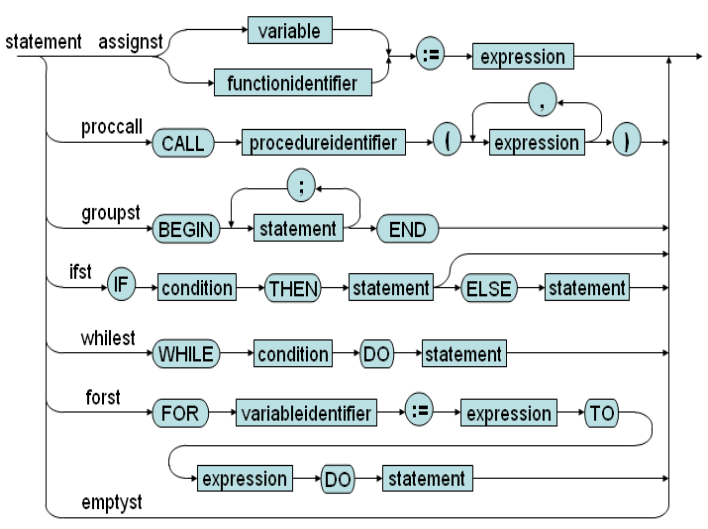
\includegraphics[width=\linewidth]{syn5.png}
					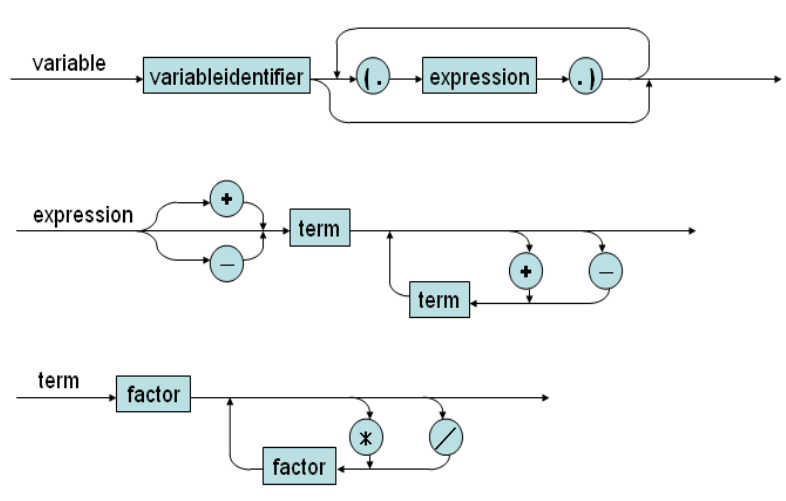
\includegraphics[width=\linewidth]{syn6.png}
					\caption{Syntax diagram 3.}
					\label{fig:syn3}
				\end{figure}
				\begin{figure}[hp]
					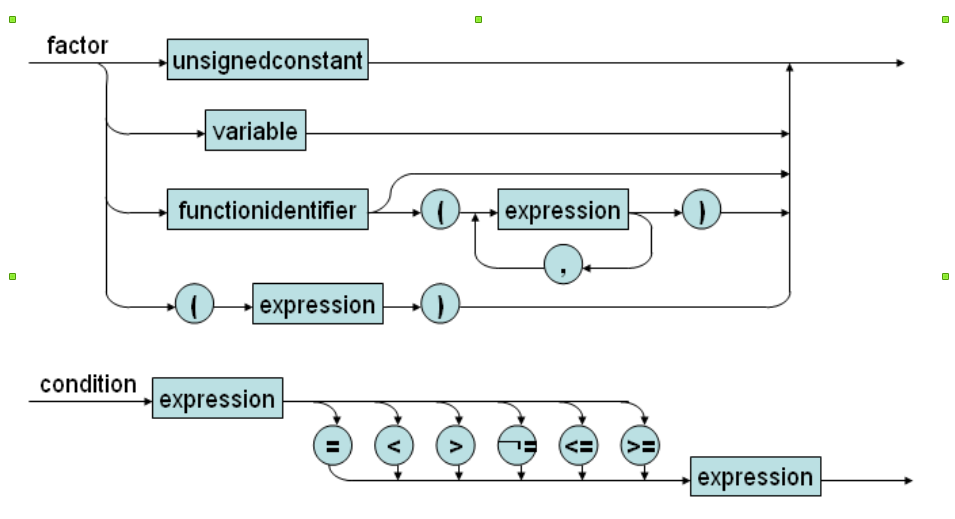
\includegraphics[width=\linewidth]{syn7.png}
					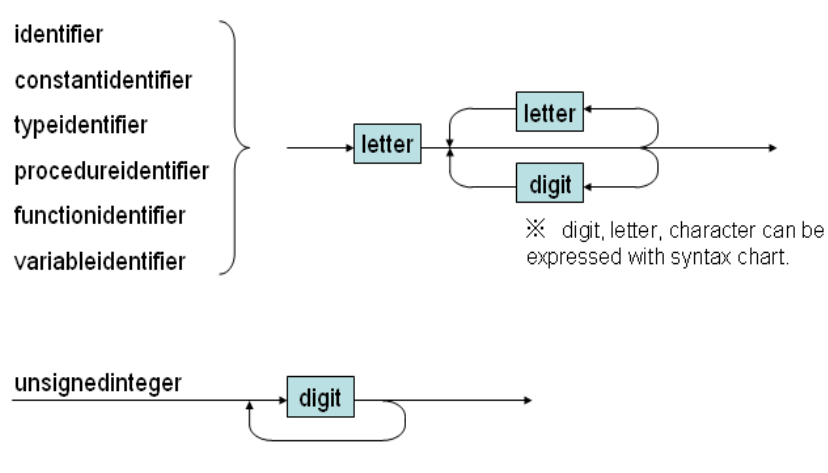
\includegraphics[width=\linewidth]{syn8.png}
					\caption{Syntax diagram 4.}
					\label{fig:syn4}
				\end{figure}

			\subsection{BNF grammar}
				\begin{enumerate}
					\item Prog ::= KW\_PROGRAM Ident SB\_SEMICOLON Block SB\_PERIOD

					\item Block  ::= KW\_CONST ConstDecl ConstDecls Block2
					\item Block  ::= Block2

					\item Block2 ::= KW\_TYPE TypeDecl TypeDecls Block3
					\item Block2 ::= Block3

					\item Block3 ::= KW\_VAR VarDecl VarDecls Block4
					\item Block3 ::= Block4

					\item Block4 ::= SubDecls Block5
					\item Block5 ::= KW\_BEGIN Statements KW\_END

					\item ConstDecls::= ConstDecl ConstDecls
					\item ConstDecls::= $\epsilon$
					\item ConstDecl ::= Ident SB\_EQUAL Constant SB\_SEMICOLON

					\item TypeDecls ::= TypeDecl TypeDecls
					\item TypeDecls ::= $\epsilon$
					\item TypeDecl ::= Ident SB\_EQUAL Type SB\_SEMICOLON

					\item VarDecls ::= VarDecl VarDecls
					\item VarDecls ::= $\epsilon$
					\item VarDecl ::= Ident SB\_COLON Type SB\_SEMICOLON

					\item SubDecls ::= FunDecl SubDecls
					\item SubDecls ::= ProcDecl SubDecls
					\item SubDecls ::= $\epsilon$

					\item FunDecl ::= KW\_FUNCTION Ident Params SB\_COLON BasicType SB\_SEMICOLON Block SB\_SEMICOLON

					\item ProcDecl ::= KW\_PROCEDURE Ident Params SB\_SEMICOLON Block SB\_SEMICOLON

					\item Params ::= SB\_LPAR Param Params2 SB\_RPAR
					\item Params ::= $\epsilon$

					\item Params2 ::= SB\_SEMICOLON Param Params2
					\item Params2 ::= $\epsilon$

					\item Param ::= Ident SB\_COLON BasicType
					\item Param ::= KW\_VAR Ident SB\_COLON BasicType
					\item Type ::= KW\_INTEGER 
					\item Type ::= KW\_CHAR 
					\item Type ::= TypeIdent 
					\item Type ::= KW\_ARRAY SB\_LSEL Number SB\_RSEL KW\_OF Type

					\item BasicType ::= KW\_INTEGER 
					\item BasicType ::= KW\_CHAR

					\item UnsignedConstant ::= Number
					\item UnsignedConstant ::= ConstIdent
					\item UnsignedConstant ::= ConstChar

					\item Constant ::= SB\_PLUS Constant2
					\item Constant ::= SB\_MINUS Constant2 
					\item Constant ::= Constant2 
					\item Constant ::= ConstChar

					\item Constant2::= ConstIdent
					\item Constant2::= Number

					\item Statements ::= Statement Statements2

					\item Statements2 ::= KW\_SEMICOLON Statement Statement2
					\item Statements2 ::= $\epsilon$

					\item Statement ::= AssignSt
					\item Statement ::= CallSt
					\item Statement ::= GroupSt
					\item Statement ::= IfSt
					\item Statement ::= WhileSt
					\item Statement ::= ForSt
					\item Statement ::= $\epsilon$ 

					\item AssignSt ::= Variable SB\_ASSIGN Expession
					\item AssignSt ::= FunctionIdent SB\_ASSIGN Expression

					\item CallSt   ::= KW\_CALL ProcedureIdent Arguments
					\item GroupSt  ::= KW\_BEGIN Statements KW\_END
					\item IfSt     ::= KW\_IF Condition KW\_THEN Statement ElseSt
					\item ElseSt   ::= KW\_ELSE statement
					\item ElseSt   ::= $\epsilon$
					\item WhileSt  ::= KW\_WHILE Condition KW\_DO Statement
					\item ForSt    ::= KW\_FOR VariableIdent SB\_ASSIGN Expression KW\_TO Expression KW\_DO Statement

					\item Arguments ::= SB\_LPAR Expression Arguments2 SB\_RLAR
					\item Arguments ::= $\epsilon$
					\item Arguments2::= SB\_COMMA Expression Arguments2
					\item Arguments2::= $\epsilon$

					\item Condition ::= Expression Condition2
					\item Condition2::= SB\_EQ Expression
					\item Condition2::= SB\_NEQ Expression
					\item Condition2::= SB\_LE Expression
					\item Condition2::= SB\_LT Expression
					\item Condition2::= SB\_GE Expression
					\item Condition2::= SB\_GT Expression   
					
					\item Expression ::= SB\_PLUS Expression2
					\item Expression ::= SB\_MINUS Expression2
					\item Expression ::= Expression2
					\item Expression2 ::= Term Expression3
					\item Expression3 ::= SB\_PLUS Term Expression3
					\item Expression3 ::= SB\_MINUS Term Expression3
					\item Expression3 ::= $\epsilon$
					
					\item Term ::= Factor Term2
					\item Term2 ::= SB\_TIMES Factor Term2
					\item Term2 ::= SB\_SLASH Factor Term2
					\item Term2 ::= $\epsilon$
					\item Factor ::= UnsignedConstant
					\item Factor ::= Variable
					\item Factor ::= FunctionApptication
					\item Factor ::= SB\_LPAR Expression SB\_RPAR
					\item Variable ::= VariableIdent Indexes
					\item FunctionApplication ::= FunctionIdent Arguments
					\item Indexes ::= SB\_LSEL Expression SB\_RSEL Indexes
					\item Indexes ::= $\epsilon$
				\end{enumerate}
		\section{Recursive descent parsing}
			\begin{itemize}
				\item Properties:
				\begin{itemize}
					\item LL(k) is the language that needs looking ahead k character to produce a valid production
           			\item Used to parse LL(1) language
           			\item Can be extended for LL(k), but very complex 
           			\item Used for other grammar can lead to infinite iteration	
				\end{itemize}				 
           		\item Recursive descent parsing:
           		\begin{itemize}
     				\item A top-down parsing method.
    				\item The term descent refers to the direction in which the  parse tree is traversed (or built). 
    				\item Use a set of mutually recursive procedures (one procedure for each nonterminal symbol). Start the parsing process by calling the procedure that corresponds to the start symbol. Each production becomes one clause in procedure 
    				\item Consider a special type of recursive-descent parsing called predictive parsing. Use a lookahead symbol to decide which production.
    			\end{itemize}
			\end{itemize}
		\section{Data structure in parser for KPL}
			\tab Like in scanner.
		\section{Parse terminal symbols}
			\textbf{void} eat(\textbf{TokenType} tokenType);\\
			Function will compare the passed tokenType to token type read in scanner (currentToken). If equals, print out the token, otherwise, report error: “missing token” at that position.
		\section{Parsing non-terminal symbols}
			\begin{itemize}
				\item \textbf{void} compileProgram(): parse main program.
      			\item \textbf{void} compileBlock(\textbf{void}): parse constant declarations then call compileBlock2.
      			\item \textbf{void} compileBlock2(\textbf{void}): parse type declarations then call compileBlock3.
      			\item \textbf{void} compileBlock3(\textbf{void}): parse variable declarations then call compileBlock4.
      			\item \textbf{void} compileBlock4(\textbf{void}):parse subroutines declarations then call compileBlock5.
      			\item \textbf{void} compileBlock5(\textbf{void}): parse statements in main function.
      			\item \textbf{void} compileConstDecls(\textbf{void}): parse constant declarations.
      			\item \textbf{void} compileConstDecl(\textbf{void}): parse a single constant declaration.
      			\item \textbf{void} compileTypeDecls(\textbf{void}): parse type declarations.
      			\item \textbf{void} compileTypeDecl(\textbf{void}): parse a single  type declaration.
      			\item \textbf{void} compileVarDecls(\textbf{void}): parse variable declarations.
      			\item \textbf{void} compileVarDecl(\textbf{void}): parse a variable declaration.
      			\item \textbf{void} compileSubDecls(\textbf{void}): parse subroutines declarations.
      			\item \textbf{void} compileFuncDecl(\textbf{void}): parse function declarations.
     			\item \textbf{void} compileProcDecl(\textbf{void}): parse procedures declarations.
      			\item \textbf{void} compileUnsignedConstant(\textbf{void}): parse unsigned constants.
      			
      			\item \textbf{void} compileConstant(\textbf{void}): parse signed constants.
      			\item \textbf{void} compileType(\textbf{void}): parse a type.
      			\item \textbf{void} compileBasicType(\textbf{void}): parse a basic type.
      			\item \textbf{void} compileParams(\textbf{void}): parse list of parameters.
      			\item \textbf{void} compileParam(\textbf{void}): parse a single parameter.
      			\item \textbf{void} compileStatements(\textbf{void}): parse all statements.
      			\item \textbf{void} compileStatement(\textbf{void}): parse a single statement.  
     			\item \textbf{void} compileAssignSt(\textbf{void}): parse an assignment statement.
      			\item \textbf{void} compileCallSt(\textbf{void}): parse a call statement.
      			\item \textbf{void} compileIfSt(\textbf{void}): parse an IF statement.
      			\item \textbf{void} compileElseSt(\textbf{void}): parse an ELSE statement.
      			\item \textbf{void} compileWhileSt(\textbf{void}): parse a WHILE statement.
      			\item \textbf{void} compileForSt(\textbf{void}): parse a FOR statement.
      			\item \textbf{void} compileArguments(\textbf{void}): parse list of arguments passed to a function or procedure.
      			\item \textbf{void} compileArguments2(\textbf{void}): parse list of arguments passed to a function or procedure.
      			\item \textbf{void} compileCondition(\textbf{void}): parse conditional expression.
      			\item \textbf{void} compileExpression(\textbf{void}): parse (+,-) of an expression then call compileExpression2
      			\item \textbf{void} compileExpression2(\textbf{void}): parse (+, - ) operators between terms then call compileExpression3
      			\item \textbf{void} compileExpression3(\textbf{void}): recursive of (+, -) operators between terms.
      			\item \textbf{void} compileTerm(\textbf{void}): compile a term, which can be composed of (*, /) of compileFactor
      			\item \textbf{void} compileTerm2(\textbf{void}) recursive procedure of (*, /) between factors.
      			\item \textbf{void} compileFactor(\textbf{void}): a factor can be a number, character, identifier .
      			\item \textbf{void} compileIndexes(\textbf{void}): parse indexes of an array.
			\end{itemize}
	\chapter{SEMANTIC ANALYSER FOR KPL}
	\newpage
		\section{Tasks of semantic analyzer}
			\tab Important tasks of a semantic analyzer:
			\begin{itemize}
				\item Produce symbol table for future references (eg. scope and type checking)
				\item Scope checking
				\item Type checking
			\end{itemize}
		\section{Symbol table designing}
			\subsection{Reason}
				\tab We need a symbol table to store information needed about every identifiers in the program. Each identifier in a program's source code is associated with information relating to its declaration or appearance in the source, such as its type, scope level and its location.
			\subsection{Design symbol table}
				\subsubsection{Data structure in symbol table}
					\begin{enumerate}
						\item struct \textbf{SymTab\_} \{\\
	  					\textbf{Object*} program;\\
	  					\textbf{Scope*} currentScope;\\
	  					\textbf{ObjectNode *}globalObjectList;\\
						\};\\
						\textbf{The data structure to represent symbol table itself, including:}
						\begin{itemize}
							\item Program: the program object
	    					\item currentScope: current scope of symbol table
	    					\item globalObjectList: store global objects such as functions: CALLI, WRITEI, etc 
						\end{itemize}
						\item \textbf{To store information about each object in program, such as main program itself, a procedure or function, a variable, a constant, etc}\\
						struct \textbf{Object\_} \{\\
  						\textbf{char} name[MAX\_IDENT\_LEN];\\
  						enum \textbf{ObjectKind} kind;\\
  						union \{\\
    					\textbf{ConstantAttributes*} constAttrs;\\
    					\textbf{VariableAttributes*} varAttrs;
    					\textbf{TypeAttributes*} typeAttrs;\\
    					\textbf{FunctionAttributes*} funcAttrs;\\
    					\textbf{ProcedureAttributes*} procAttrs;\\
    					\textbf{ProgramAttributes*} progAttrs;\\
    					\textbf{ParameterAttributes*} paramAttrs;\\
 						\};\};	\\
 						\item \textbf{Kinds of object (a variable object, a constant object, etc)}\\
 						enum \textbf{ObjectKind} \{\\
  						OBJ\_CONSTANT,\\
  						OBJ\_VARIABLE,\\
  						OBJ\_TYPE,\\
  						OBJ\_FUNCTION,\\
  						OBJ\_PROCEDURE,\\
  						OBJ\_PARAMETER,\\
  						OBJ\_PROGRAM\\
						\};
						\item \textbf{Kinds of parameter: value or reference type}\\
						enum \textbf{ParamKind} \{\\
  						PARAM\_VALUE,
  						PARAM\_REFERENCE
						\};
						\item \textbf{To store information about a scope, including:}
						\begin{itemize}
							\item objList: objects in the scope
    						\item Owner: function or procedure has that scope
    						\item Outer: the outer scope of it
						\end{itemize}
						struct \textbf{Scope\_} \{\\
  						\textbf{ObjectNode *}objList;\\
  						\textbf{Object *}owner;\\
  						struct \textbf{Scope\_ *}outer;\\
						\};
						\item \textbf{A linked list to represent list of objects}\\
						struct \textbf{ObjectNode\_} \{\\
  						\textbf{Object *}object;\\
  						struct \textbf{ObjectNode\_ *}next;\\
						\};
						\item \textbf{To store typical attributes of each type: e.g a constant type must have a constant value, a function type must have a parameter list, a return type, and own a scope}\\
						struct \textbf{ConstantValue\_} \{\\
  						enum \textbf{TypeClass} type;\\
  						union \{\\
    					\textbf{int} intValue;\\
    					\textbf{char} charValue;\\
  						\};\};\\

						typedef struct \textbf{ConstantValue\_} ConstantValue;\\

						struct \textbf{Scope\_};\\
						struct \textbf{ObjectNode\_};\\
						struct \textbf{Object\_};\\
						
						struct \textbf{ConstantAttributes\_} \{\\
						  \textbf{ConstantValue*} value;\\
						\};
						
						struct \textbf{VariableAttributes\_} \{\\
						  \textbf{Type *}type;\\
						  struct \textbf{Scope\_ *}scope;\\
						\};\\
						
						struct \textbf{TypeAttributes\_} \{\\
						  \textbf{Type *}actualType;\\
						\};\\
						
						struct \textbf{ProcedureAttributes\_} \{\\
						  struct \textbf{ObjectNode\_ *}paramList;\\
						  struct \textbf{Scope\_*} scope;\\
						\};\\
						
						struct \textbf{FunctionAttributes\_} \{\\
						  struct \textbf{ObjectNode\_ *}paramList;\\
						  \textbf{Type*} returnType;\\
						  struct \textbf{Scope\_ *}scope;\\
						\};\\
						
						struct \textbf{ProgramAttributes\_} \{\\
						  struct \textbf{Scope\_ *}scope;\\
						\};\\
						
						struct \textbf{ParameterAttributes\_} \{\\
						  enum \textbf{ParamKind} kind;\\
						  \textbf{Type*} type;\\
						  struct \textbf{Object\_ *}function;\\
						\};\\
						
						typedef struct \textbf{ConstantAttributes\_} ConstantAttributes;\\
						typedef struct \textbf{TypeAttributes\_} TypeAttributes;\\
						typedef struct \textbf{VariableAttributes\_} VariableAttributes;\\
						typedef struct \textbf{FunctionAttributes\_} FunctionAttributes;\\
						typedef struct \textbf{ProcedureAttributes\_} ProcedureAttributes;\\
						typedef struct \textbf{ProgramAttributes\_} ProgramAttributes;\\
						typedef struct \textbf{ParameterAttributes\_} ParameterAttributes;
					\end{enumerate}
				\subsubsection{Functions in symbol table}
					\begin{itemize}
						\item \textbf{Object*}createProgramObject(\textbf{char *}programName): create a program object.
						\item \textbf{Object*} createConstantObject(\textbf{char *}name): create a constant object.
						\item \textbf{Object*} createTypeObject(\textbf{char *}name): create a type object.
						\item \textbf{Object*} createVariableObject(\textbf{char *}name): create a variable object.
						\item \textbf{Object*} createFunctionObject(\textbf{char *}name): create a function object.
						\item \textbf{Object*} createProcedureObject(\textbf{char *}name): create a procedure object.
						\item \textbf{Object*} createParameterObject(\textbf{char *}name, enum \textbf{ParamKind} kind, \textbf{Object*} owner): create a parameter object.
						
						\item \textbf{Type*} makeIntType(\textbf{void}): create an integer type.
						\item \textbf{Type*} makeCharType(\textbf{void}): create a character type.
						\item \textbf{Type*} makeArrayType(\textbf{int} arraySize, \textbf{Type*} elementType): create an array type.
						\item \textbf{Type*} duplicateType(\textbf{Type*} type): copy type.
						int compareType(\textbf{Type*} type1, \textbf{Type*} type2): compare type
						
						\item \textbf{ConstantValue*} makeIntConstant(\textbf{int} i): create an integer constant.
						\item \textbf{ConstantValue*} makeCharConstant(\textbf{char} ch): create a character constant.
						\item \textbf{ConstantValue*} duplicateConstantValue(\textbf{ConstantValue*} v): copy a constant.
						
						\item \textbf{Scope*} createScope(\textbf{Object*} owner, \textbf{Scope*} outer): create a scope.
						\item \textbf{Object*} findObject(\textbf{ObjectNode *}objList, \textbf{char *}name): find object with specific name in an object list.
					\end{itemize}
		\section{Verify scoping rules}
			\subsection{Checking fresh identifier}
				\tab We determine if an identifier is not declared yet, by function \textbf{void} checkFreshIdent(\textbf{char *}name). If the identifier is already declared, function findObject will return an non-null value\\
				\textbf{void} checkFreshIdent(\textbf{char *}name) \{\\
  				if (findObject(symtab-$>$currentScope-$>$objList, name) != \textbf{NULL})
    			error(ERR\_DUPLICATE\_IDENT, currentToken-$>$lineNo, currentToken-$>$colNo);\\
\}
			\subsection{Checking declared identifier}
				\begin{itemize}
					\item \textbf{Object*} checkDeclaredIdent(\textbf{char *}name): check declared identifiers: (identifier is already declared or not. If declared return identifier object, else return \textbf{NULL})
					\item \textbf{Object*} checkDeclaredConstant(\textbf{char *}name): check declared constants
					\item \textbf{Object*} checkDeclaredType(\textbf{char *}name): check declared identifiers
					\item \textbf{Object*} checkDeclaredVariable(\textbf{char *}name): check declared variables
					\item \textbf{Object*} checkDeclaredFunction(\textbf{char *}name): check declared functions
					\item \textbf{Object*} checkDeclaredProcedure(\textbf{char *}name): check declared procedure
					\item \textbf{Object*} checkDeclaredLValueIdent(\textbf{char *}name): check declared LValue
				\end{itemize}
		\section{Type checking}
			\subsection{Reason}
				\begin{itemize}
					\item Check the consistency between declaration and usage of identifiers
					\item Check specific requirements in some statement (e.g. LValue in assign statement
				\end{itemize}
			\subsection{Functions}
				\begin{itemize}
					\item \textbf{void} checkIntType(\textbf{Type*} type): check if type is integer
					\item \textbf{void} checkCharType(\textbf{Type*} type): check if type is character	
					\item \textbf{void} checkArrayType(\textbf{Type*} type): check if type is array type.
					\item \textbf{void} checkBasicType(\textbf{Type*} type): check if type is basic type.
					\item \textbf{void} checkTypeEquality(\textbf{Type*} type1, \textbf{Type*} type2): check for equality of types, if not, report an error message.
				\end{itemize}

					
\end{document}